\documentclass[preprint,numbers]{sigplanconf}

\newif\ifanonymous

%\anonymoustrue
\anonymousfalse

\usepackage{amsmath}
\usepackage{graphicx}
\usepackage{xcolor}
\usepackage{xspace}
\usepackage{verbatim}
\usepackage{listings}
\lstset{%
	basicstyle=\scriptsize\ttfamily,
	language={Haskell},
	inputencoding=utf8,
	breaklines=true,
	prebreak = \raisebox{0ex}[0ex][0ex]{\ensuremath{\hookleftarrow}},
	morekeywords={},
	deletekeywords={Num},
	keywordstyle=\color[rgb]{0,0,1},             % keywords
	commentstyle=\color[rgb]{0.133,0.545,0.133}, % comments
	stringstyle=\color[rgb]{0.627,0.126,0.941},  % strings
	escapechar=@,
}
\usepackage{array}
\usepackage{tikz}
\usetikzlibrary{arrows,positioning,
  shapes.multipart,
  matrix,
  positioning,
  shapes.callouts,
  shapes.arrows,
  calc}

\newcommand{\TODO}[1]{{\color{black!10!blue}TODO #1}}
\newcommand{\mydraft}[1]{{\color{black!50!green}#1}}
\newcommand{\mywrong}[1]{{\color{black!10!red}#1}}

\DeclareMathOperator{\where}{where}
\DeclareMathOperator{\bxget}{get}
\DeclareMathOperator{\bxput}{put}
\DeclareMathOperator{\bxcreate}{create}
\DeclareMathOperator{\dput}{dput}
\DeclareMathOperator{\dcreate}{dcreate}
\DeclareMathOperator{\data}{data}
\DeclareMathOperator{\shape}{shape}
\DeclareMathOperator{\recover}{recover}
\DeclareMathOperator{\locs}{locs}

\begin{document}

\special{papersize=8.5in,11in}
\setlength{\pdfpageheight}{\paperheight}
\setlength{\pdfpagewidth}{\paperwidth}

\conferenceinfo{CONF 'yy}{Month d--d, 20yy, City, ST, Country}
\copyrightyear{20yy}
\copyrightdata{978-1-nnnn-nnnn-n/yy/mm}
\copyrightdoi{nnnnnnn.nnnnnnn}

% Uncomment the publication rights you want to use.
%\publicationrights{transferred}
%\publicationrights{licensed}     % this is the default
%\publicationrights{author-pays}

%\titlebanner{banner above paper title}        % These are ignored unless
%\preprintfooter{short description of paper}   % 'preprint' option specified.

\title{The Under-Appreciated Put: Implementing Delta-Alignment in BiGUL}
\subtitle{Functional Pearl}

\ifanonymous
\authorinfo{}{}{}
\else
\authorinfo{Jorge Mendes}
           {HASLab, INESC TEC \& Universidade do Minho, Portugal}
           {jorgemendes@di.uminho.pt}
%\authorinfo{Name2\and Name3}
%           {Affiliation2/3}
%           {Email2/3}
\fi

\maketitle

\begin{abstract}
  \TODO{Ideas to express: BX in the put direction is precise; more concepts can
  be described. An example of such concept is alignment.}
\end{abstract}

\category{CR-number}{subcategory}{third-level}

% general terms are not compulsory anymore,
% you may leave them out
\terms
term1, term2

\keywords
keyword1, keyword2


%%%
%%% Introduction
%%%
\section{Introduction}

Several approaches exist to help dealing with specific situations when
developing software. One such approach consists in the use of bidirectional
transformation (BX) mechanisms to maintain consistency between two pieces of
related information.

Some work on BXs emerges from the view-update problem, where a view is generated
from a source database and consistency must be kept between these two artefacts.
If the view suffers changes, these should be reflected in the source database.

The \emph{lens} framework~\cite{Greenwald2003} emerged to solve similar
problems, where a \emph{get} function creates a abstract view from a concrete
source, and a \emph{put} function provides an updated source using the original
source and the modified view.

To define a BX system, one has to provide a \emph{get} and a \emph{put}
functions, ensuring that some properties are statisfied by this pair of
functions. These properties ensure the \emph{well-behavedness} of the BX system.

Research was done in order to derive a suitable \emph{put} for a given
\emph{get} in order to help the development of BXs. This has some limitations,
since the \emph{put} direction is usually the problematic one.

An example of a get program is the projection of a map structure, selecting its
key and part of its value:
%
\[ \mathcal M (K, (V_1, V_2)) \longrightarrow \mathcal M (K, V_1) \]
%
This has several possible \emph{put} functions that would satisfy the
\emph{well-behavedness} properties. One can annotate the transformation in order
to select a way to perform the \emph{put} operation:
%
\[ \mathcal M (K, (V_1, V_2)) \xrightarrow{\text{\small best match on \(K\)}} \mathcal M (K, V_1) \]
%
This provides information on how to align the elements in the \emph{put}
direction. But it is not enough: how to deal with new elements? One can provide
another annotation:
%
\[ \mathcal M (K, (V_1, V_2 = v_2)) \xrightarrow{\text{\small best match on \(K\)}} \mathcal M (K, V_1) \]
%
where \(v_2\) is a default value for type \(V_2\).

Another approach is writing the \emph{put} function. This is more difficult than
writing the \emph{get} function, but it removes the need for extra annotations.
The \emph{put} function has access to both the original source and the modified
view, i.e., all the possible information available to write a program that
provides an updated source. The program, in this example, includes the logic
that leads to the alignment strategy and the default value to use for new
elements. Moreover, an unique \emph{get} function can be derived from this
\emph{put}.
%
\[ \mathcal M (K, (V_1, V_2)) \longleftarrow \mathcal M (K, (V_1, V_2)) \times \mathcal M (K, V_1) \]

% Motivation for delta-based alignment.
This example continues to have some drawbacks. The key-based alignment might not
reflect the operations performed to the view, resulting in an incorrect
alignment. Having information about the operations performed to the view, it
should be possible to provide a relation of the elements from the original view
that are also present in the modified view. Using this relation, or
\emph{delta}, it is possible to precisely align the elements in the modified
view with the ones in the original source for the \emph{put} operation.
%
\[ \mathcal M (K, (V_1, V_2)) \longleftarrow \mathcal M (K, (V_1, V_2)) \times \mathcal M (K, V_1) \times \Delta \]

\TODO{Goal of the paper. Show that defining the \emph{put} direction has its
benefits and can be more intuitive for certain operations. Moreover, it shows
how to use additional information, namely the delta, that isn't defined in the
put operation, but in is given at runtime instead.}

In the next sections, an overview on bidirectional transformations and the
alignment problem is provided. Then, putback-based bidirectional transformation
techniques are presented, followed by an implementation of alignment using such
technique.


%%%
%%% Bidirectional Transformations
%%%
\section{Bidirectional Transformations}

A successful language to specify BX systems is the \emph{lenses}
language~\cite{Greenwald2003}. A lens \(l : S \leftrightarrow V\), with source
type \(S\) and view type \(V\), is composed by two functions:
%
\begin{align*}
  \bxget &:: S \rightarrow V\\
  \bxput &:: S \rightarrow V \rightarrow S
\end{align*}
%
The \emph{get} function extracts a view from a source and the \emph{put}
function updates the original source with information from the new view.

When developing a BX system, one expects it to be \emph{well-behaved}, i.e.,
that performing certain actions should provide a stable result. One of these
actions is updating a source with an unmodified view of such source, which
should result in the same source. Another action is getting the view after
updating a source, which should result in the same view used for the update.
From these actions and respective results, two laws were defined:
\textsc{PutGet}, for the former action; and, \textsc{GetPut}, for the latter.

For the lenses framework, in order a BX system to be considered
\emph{well-behaved}, the following two laws must be ensured:
%
\begin{align*}
  \bxget \left(\bxput s~v\right) = v
    \tag{\sc GetPut}\label{eq:getput}\\
  \bxput s\,\left(\bxget s\right) = s
    \tag{\sc PutGet}\label{eq:putget}
\end{align*}
%
The \ref{eq:getput} law states that after performing an update to the original
source, the view obtained from this result should be the same as the one used to
perform the update. The \ref{eq:putget} law states that updating the source with an
unchanged view should result in the original source.

\noindent\TODO{
  \begin{itemize}
    \item get is easier to write than put. When writing get, a put can be
      derived, but, since it may be not unique, some assumptions are made, and
      in some cases update policies must be provided.
      Where is this information available?
  \end{itemize}
}

%%
%% TODO (maybe)
%% very well-behaved lenses (it is worth to mention?)
%%  - the create function
%%  - variations from other languages (matching lenses, delta lenses,~\dots)
%%


%%%
%%% The Alignment Problem
%%%
\section{The Alignment Problem}

Alignment consists in matching elements in the source container with elements in
the source container. When modifying a view, the elements in a container might
be modified, e.g., new elements are added, others are deleted, or some are moved
within the container. Many examples of containers exist, with lists and trees
being the more common.

\begin{figure}[ht]
  \centering
  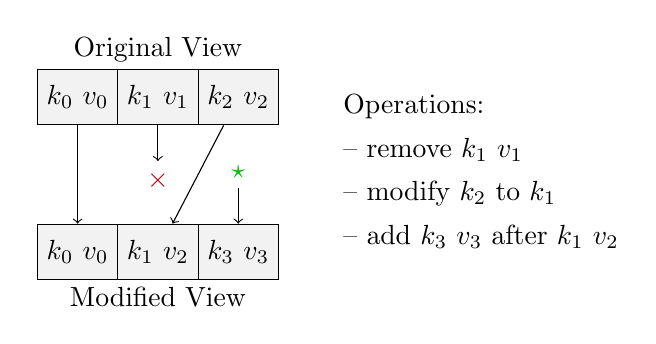
\begin{tikzpicture}[
  array/.style={
    matrix of nodes,
    nodes={draw, minimum size=7mm, fill=gray!10},
    column sep=-\pgflinewidth,
    row sep=0.5mm,
    nodes in empty cells
  },
  operations/.style={
    rectangle split,
    rectangle split parts=#1,
    rectangle split part align=left
  }]

%% original source
%\matrix[array, anchor=west] (s0) { \(k_0~v_0\) & \(k_1~v_1\) & \(k_2~v_2\) \\ };
%\node[above = -1ex of s0] (s0label) {Source};

% original view
\matrix[array] (v0) { \(k_0~v_0\) & \(k_1~v_1\) & \(k_2~v_2\) \\ };
\node[above = -1ex of v0] (v0label) {Original View};

% modified view
\matrix[array, below = 1cm of v0] (v1) { \(k_0~v_0\) & \(k_1~v_2\) & \(k_3~v_3\) \\ };
\node[below = -1ex of v1] (v1label) {Modified View};

% changes in the view
\draw[->] (v0-1-1) -> (v1-1-1);
\node[below = 3ex of v0-1-2] (v0del) {\color{black!25!red} \(\times\)};
\draw[->] (v0-1-2) -> (v0del);
\draw[->] (v0-1-3) -> (v1-1-2);
\node[above = 3ex of v1-1-3] (v1add) {\color{black!25!green} \(\star\)};
\draw[->] (v1add) -> (v1-1-3);

% list of operations
\node[operations=4,right=1cm of v1add]
  (operations)
  {%
    Operations:
    \nodepart{two} -- remove \(k_1~v_1\)
    \nodepart{three} -- modify \(k_2\) to \(k_1\)
    \nodepart{four} -- add \(k_3~v_3\) after \(k_1~v_2\)
  }; 

\end{tikzpicture}

  \caption{Example of a view, the changes applied to it, and the obtained
  result. Other sets of operations can result in the same view.}
  \label{fig:alignment}
\end{figure}

Unexpected results can be obtained when container elements are not properly
aligned. Most of these issues are consequences of the alignment approach
selected, which include the following ones:
%
% Kinds of alignments
% - [implicitly] positional
% - arbitrary algorithm
% - delta-based
% - operation-based
%
\begin{itemize}
  \item positional update;
  \item use of an arbitrary matching algorithm (e.g., best match);
  \item delta-based alignment; and,
  \item operation-based BX.
\end{itemize}

A positional update of the elements removes elements at the start/end of the source
if it contains more elements than the view, or adds new elements at the
start/end of the source if the view have more elements. Here, start/end is an
arbitrary position within the source. The move of elements is not taken into
account. Using the example in Fig.~\ref{fig:alignment}, a positional update
would be equivalent to a modification of \(v_1\) to \(v_2\), and a change of
\(k_2~v_2\) to \(k_3~v_3\). Thus, the alignment does not reflect the operations
performed to the view.

Using an algorithm to match elements of the original source with elements of the
new view can provide more precision than the positional update. A common
strategy is key-based matching, where a key is used to identify the elements
in the container. With the example in Fig.~\ref{fig:alignment}, one can use the
\(k\) part of the element as a key, resulting in an alignment equivalent to the
modification of \(v_1\) to \(v_2\), the removal of \(k_2~v_2\) and the addition
of \(k_3~v_3\). This alignment also does not reflect the operations performed to
the view, but it is closer than the positional update.

Using information about changes in the view (i.e., \emph{deltas}) is one of the
approaches so that
the elements can be matched accurately between the original source and the
new view. This can be implemented in distinct fashions, one of them identifying
the relation of the elements in the original view with the ones in the modified
view. The elements that are not in this relation were either deleted (if not
present in the modified view) or added (if not present in the original view).

Finally, it is also possible to work with operations, matching operations
performed on the view with operations to be performed on the source.

The first two approaches might not reflect the actual changes performed to the
view, which can introduce some misalignment of the elements of the view with the
source ones. Moreover, these approaches are implicit in some frameworks, or
require additional annotations in the programs. On the other hand, the last two
options use information of the
actual changes or operations performed, resulting in a precise alignment.
However, this information is not always available thus preventing the use of
the last two precise options in some situations. Furthermore, these approaches
differ from the traditional lenses, where more information should be provided
(in the case of the deltas), or the complete system logic is flipped and the BX
system works with operations instead of the usual artefacts.

\TODO{What BX frameworks changed in order to allow alignment strategies. E.g.,
matching lenses and the resources/complements/chunks.}

\begin{comment}

\noindent\TODO{
\begin{itemize}
  \item Background/related work to understand the work presented in this paper.
  \item From ``Deltas over Polymorphic Inductive Types''
    \begin{itemize}
      \item Functors
      \item Positions
      \item Deltas
    \end{itemize}
  \item Shapely type functions:
    \begin{itemize}
      \item shape
      \item data
      \item recover
    \end{itemize}
\end{itemize}
}

\noindent\TODO{
\begin{itemize}
  \item Description of mapping elements from the view to elements on the source.
  \item In the get direction, position of elements does not change. There is a
    one-to-one mapping.
  \item In the put direction, the source is recovered using its shape and the
    updated data from the original source with the new view using the
    information from the delta.
\end{itemize}
}

\end{comment}


%%%
%%% Putback-Based Bidirectional Transformations
%%%
\section{Putback-Based Bidirectional Transformations}

An under-appreciated fact about well-behaved lenses is that \emph{put} completely determines the behavior of the corresponding \emph{get} --- that is, given a \emph{put} function and two \emph{get} functions each of which forms a well-behaved lens when paired with the \emph{put} function, it must be the case that the two \emph{get} functions are pointwise equal. This fact was already noted by Foster in his PhD thesis~\cite{Foster2009} but had remained neglected until people dug up this idea and started exploring the possibility of specifying BXs in terms of \emph{put} \TODO{citations}.

Intuitively, think of a BiGUL program of type \lstinline{BiGUL s v} as describing how to manipulate a state consisting of a source component of type~\lstinline{s} and a view component of type~\lstinline{v}; the goal is to copy all information in the view to proper places in the source.
In the simplest case, the view has type \lstinline{()} and contains no information, and we can use \lstinline{Skip :: BiGUL s ()} to leave the source unchanged;
another simple case is when the view has the same type as the source, and we can use \lstinline{Replace :: BiGUL s s} to replace the entire source with the view.
BiGUL programs compose --- for example, when both the source and the view are pairs, we can use
\begin{lstlisting}
Prod :: BiGUL s v -> BiGUL s' v' ->
        BiGUL (s, s') (v, v')
\end{lstlisting}
to compose two BiGUL programs on the left and right components respectively.
Of course, in most cases the source and view are in more complex forms, and we should somehow transform and decompose them into simpler forms before we can use \lstinline{Skip}, \lstinline{Replace}, or \lstinline{Prod}; this is usually done using two ``rearrangement'' operations on the source and view respectively:
We can use the source rearranging operation
\begin{lstlisting}
$(rearrS [| f |]) :: BiGUL s' v -> BiGUL s v
\end{lstlisting}
where \lstinline{f}~is a ``simple'' $\lambda$-expression of type \lstinline{s -> s'} for extracting from the source of type~\lstinline{s} a (usually smaller) source of type~\lstinline{s'} before performing further updates on the extracted source, or dually the view rearranging operation
\begin{lstlisting}
$(rearrV [| g |]) :: BiGUL s v' -> BiGUL s v
\end{lstlisting}
where the ``simple'' $\lambda$-expression \lstinline{g} should have type \lstinline{v -> v'}, and is used to transform the view from type~\lstinline{v} to type~\lstinline{v'} before performing further updates.

Most expressiveness of BiGUL comes from its \lstinline{Case} operation for performing case analysis:
\begin{lstlisting}
Case :: [(s -> b -> Bool, Branch s v)] -> BiGUL s v
\end{lstlisting}
\lstinline{Case} takes a list of pairs whose first component is a boolean predicate on both the source and the view, and whose second component is a ``branch''.
A branch can be a ``normal'' branch, in which case it is a BiGUL program of type \lstinline{BiGUL s v}, or an ``adaptive'' branch, in which case it is a Haskell function of type \lstinline{s -> v -> s}.
The semantics of \lstinline{Case} is largely as people would expect: executing the first branch whose associated predicate evaluates to true on the current state, and performing further updates when this branch is normal.
More interestingly, when the chosen branch is adaptive, the source will be replaced by the result of evaluating the associated function on the current state and the whole \lstinline{Case} will be executed again.

%%%
%%% Alignment as a put Program
%%%
\section{Alignment as a \emph{put} Program}

Alignment is a process performed when the source is updated with the new view.
Thus, it falls naturally in the process of writing a \emph{put} program.

\noindent\TODO{More text motivating writing alignment in a put program.
Introduction for the next subsections.}

\subsection{Positional Update for Lists}

An implementation of positional mapping on lists is presented in
Listing~\ref{lst:posmapl}. This implementation receives a function to create new
source elements when a new view element is added, and a BiGUL program to perform
the element update. It is specified for the several situations that can occur:
\begin{enumerate}
  \item\label{item:posmap1} both view and source are empty;
  \item\label{item:posmap2} view is empty but source has elements;
  \item\label{item:posmap3} both view and source have elements;
  \item\label{item:posmap4} view has elements but source is empty.
\end{enumerate}

The content of both the view and the source are checked with the \emph{case}
construct, where each of the alternatives checks for one of the possible
situations following the given order. In situation~\ref{item:posmap1}, a
\emph{skip} is performed since
there are no elements to update. In situation~\ref{item:posmap2}, the content of
the source is discarded, and a new empty source is used to match the empty view.
This results in the removal of elements that are not present in the view. In
situation~\ref{item:posmap3}, normal element wise update is performed. Finally,
in situation~\ref{item:posmap4}, the empty source is transformed in a new source
with only one element that is not used since it is replace by the value from the
view.

\begin{lstlisting}[caption={Positional mapping of lists.},label={lst:posmapl}]
mapL :: (v -> s)
     -> BiGUL s v
     -> BiGUL [s] [v]
mapL c u = Case
  [ $(normalSV [p| [] |] [p| [] |])$
      $(rearrV [| \ [] -> () |]) Skip
  , $(adaptiveV [p| [] |])$ \ _ _ -> []
  , $(normalSV [p| (_ : _) |] [p| (_ : _) |])$
      $(rearrV [| \ (v:vs) -> (v, vs) |])$
        $(rearrS [| \(s:ss) -> (s, ss) |])$
          u `Prod` mapL c u
  , $(adaptiveV [p| (_ : _) |])$
    \ _ (v : _) -> [c v]
  ]
\end{lstlisting}

Positional mapping does not take into account changes in the model, except for
added or deleted elements that are dealt with at the end of the new source.
However, it is useful to map elements when the source is modified to correspond
to the view in the alignment process.

\subsection{Containers as Shape and Data}

\citet{Pacheco2012} rely on types with explicit notion of shape and data, a
property provided by polymorphic data types in functional programming.

Employing this concept, one can abstract from the shapes of both source and
view, and just take the data into account for the alignment process.

\TODO{Improve description. Information about $\shape$, $\data$, $\recover$, and
$\locs$ (used in getId).}

\subsection{Delta-Alignment for Lists}

Thus, deltas are inserted into the BiGUL alignment program in order to obtain a
precise alignment (see Listing~\ref{lst:align0}).

\begin{lstlisting}[caption={Delta-based alignment function for lists.},label={lst:align0}]
align' :: BiGUL a b
       -> (b -> a)
       -> BiGUL ([a], Delta [b] [b]) [b]
align' b c = Case
  [ $(normal [| \(_, d) v -> d == getId v |])$
      $(rearrS [| \(s, _) -> s |])$ mapL (const undefined) b
  , $(adaptiveS [| const True |])$
      \(s,d) v -> let s' = putMapD c s v d
                  in (s', getId v)
  ]
\end{lstlisting}

The alignment process is done in two steps:
%
\begin{enumerate}
  %\item Creation of new elements and removal of deleted elements.
  \item Modification of the source aligning to the view using a delta.
  \item Positional update.
\end{enumerate}
%
An alternative case statement is used to check which of these two steps are to
be performed. This is done based on the changes performed on the view: if no
changes were performed, the delta maps each element's position to the same
position (the identity delta, Listing~\ref{lst:getid}); otherwise, a
transformation is performed on the source to rearrange the elements based on the
delta, create missing view elements, and
delete no longer existent view elements.

\begin{lstlisting}[caption={Get identity delta.},label={lst:getid}]
getId :: [a] -> Delta [a] [a]
getId = map (id /\ id) . Set.elems . locs
\end{lstlisting}

\TODO{Listing~\ref{lst:putmapd} does the put direction:}
\begin{flalign*}
  \bxget s \hspace{2ex} &= S \bxget_l s &\\
  \bxput s\, v          &= \recover \left(\shape v, \dput \cup \dcreate\right) \\
  \where \hspace{-2ex}&\hspace{3ex}\dput = \bxput_l \circ \langle \data v, \data s \circ d\rangle\\
         \hspace{-2ex}&\hspace{3ex}\dcreate = (\bxcreate_l \circ \data v) \circ (id - \delta\dput)
\end{flalign*}

\begin{lstlisting}[caption={Mapping of elements between to containers of the same type using a delta.},label={lst:putmapd}]
putMapD
 :: (b -> a) -- Function to create a missing source
 -> [a]           -- Source
 -> [b]           -- View
 -> Delta [b] [b] -- View delta
 -> [a]
putMapD c s v dV = fst (traverse aux (v,0))
 where aux (vi, i) | Set.size js > 0 = (si, succ i)
                   | otherwise = (c vi, succ i)
         where js = rngOf i d
               si = data_(s) !! (Set.findMin js)
               d = Set.fromList dV
\end{lstlisting}

\begin{lstlisting}[caption={Delta-based alignment function for lists.},label={lst:align1}]
align :: BiGUL a b
      -> (b -> a)
      -> Delta [b] [b]
      -> BiGUL [a] [b]
align b c d = emb g p
  where g s   = get (align' b c) (s, getId s)
        p s v = fst (put (align' b c) (s, d) v)
\end{lstlisting}

It is possible to make minor changes to the \lstinline!align! function to
implement other kinds of alignments, e.g., key-based
(Listing~\ref{lst:keyalign}).

\begin{lstlisting}[caption={Key-based alignment function for lists.},label={lst:keyalign}]
keyAlign
  :: (Shapely s, s ~ [], Eq b, Eq k)
  => BiGUL a b         -- Inner BiGUL program
  -> (b -> a)          -- Create function
  -> (a -> k)          -- Source key
  -> (b -> k)          -- View key
  -> BiGUL (s a) (s b)
keyAlign b c sk vk = emb g p
  where g s   = get (pAlign' b c) (s, getId s)
        p s v = fst $ put (pAlign' b c)
                          (s, keyDelta sk vk s v) v
\end{lstlisting}

The \lstinline!keyAlign! function, instead of receiving the delta, receives two
functions to get the key component of the view and the source, respectively.
Then, using the original source and the modified view, another function is used
to infer a delta --- \lstinline!keyDelta!, Listing~\ref{lst:keydelta}.

\begin{lstlisting}[caption={Calculation of deltas using key-based alignment.},label={lst:keydelta}]
keyDelta
  :: (Shapely s, Eq k)
  => (a -> k)          -- Source key
  -> (b -> k)          -- View key
  -> s a               -- Source
  -> s b               -- View
  -> Delta (s a) (s b)
keyDelta sk vk ss vs =
  [ (sp, vp) | (s, sp) <- sps, (v, vp) <- vps
                             , sk s == vk v   ]
  where sps = zip (data_ ss) [0..]
        vps = zip (data_ vs) [0..]
\end{lstlisting}

%%% Generic Implementation for Container/Shapely Types
\subsection{Generic Implementation for Container/Shapely Types}

\noindent\TODO{
\begin{itemize}
  \item A generalization of the implementation for lists.
    \begin{itemize}
      \item This is currently implemented with any container as the source and a
        list as a view.
    \end{itemize}
\end{itemize}
}


%%%
%%% Conclusion
%%%
\section{Conclusion}

\TODO

%\appendix
%\section{Appendix Title}
%
%This is the text of the appendix, if you need one.

%\acks
%
%Acknowledgments, if needed.

% We recommend abbrvnat bibliography style.

\bibliographystyle{abbrvnat}
\bibliography{references}

%% The bibliography should be embedded for final submission.
%
%\begin{thebibliography}{}
%\softraggedright
%
%\bibitem[Smith et~al.(2009)Smith, Jones]{smith02}
%P. Q. Smith, and X. Y. Jones. ...reference text...
%
%\end{thebibliography}

\end{document}
